\section{Analizator sygnałów logicznych - test zaprojektowanego systemu}
    W celu przetestowania układu należy wygenerować odpowiednio duży wektor testowy,
    pozwalający na rzetelne sprawdzenie wszystkich możliwych kombinacji.
    Jednocześnie wektor ten powinien był w miarę możliwości prosty do sprawdzenia.
    Dlatego też jako wektor testowy wykorzystano licznik binarny, który z każdym stanem powinien rosnąć o dokładnie \textit{,,1''}.

    Poniżej przedstawiono zdjęcie aplikacji wyświetlającej 512 próbek odebranych za pomocą analizatora.
    \begin{figure}[!ht]
        \centering
        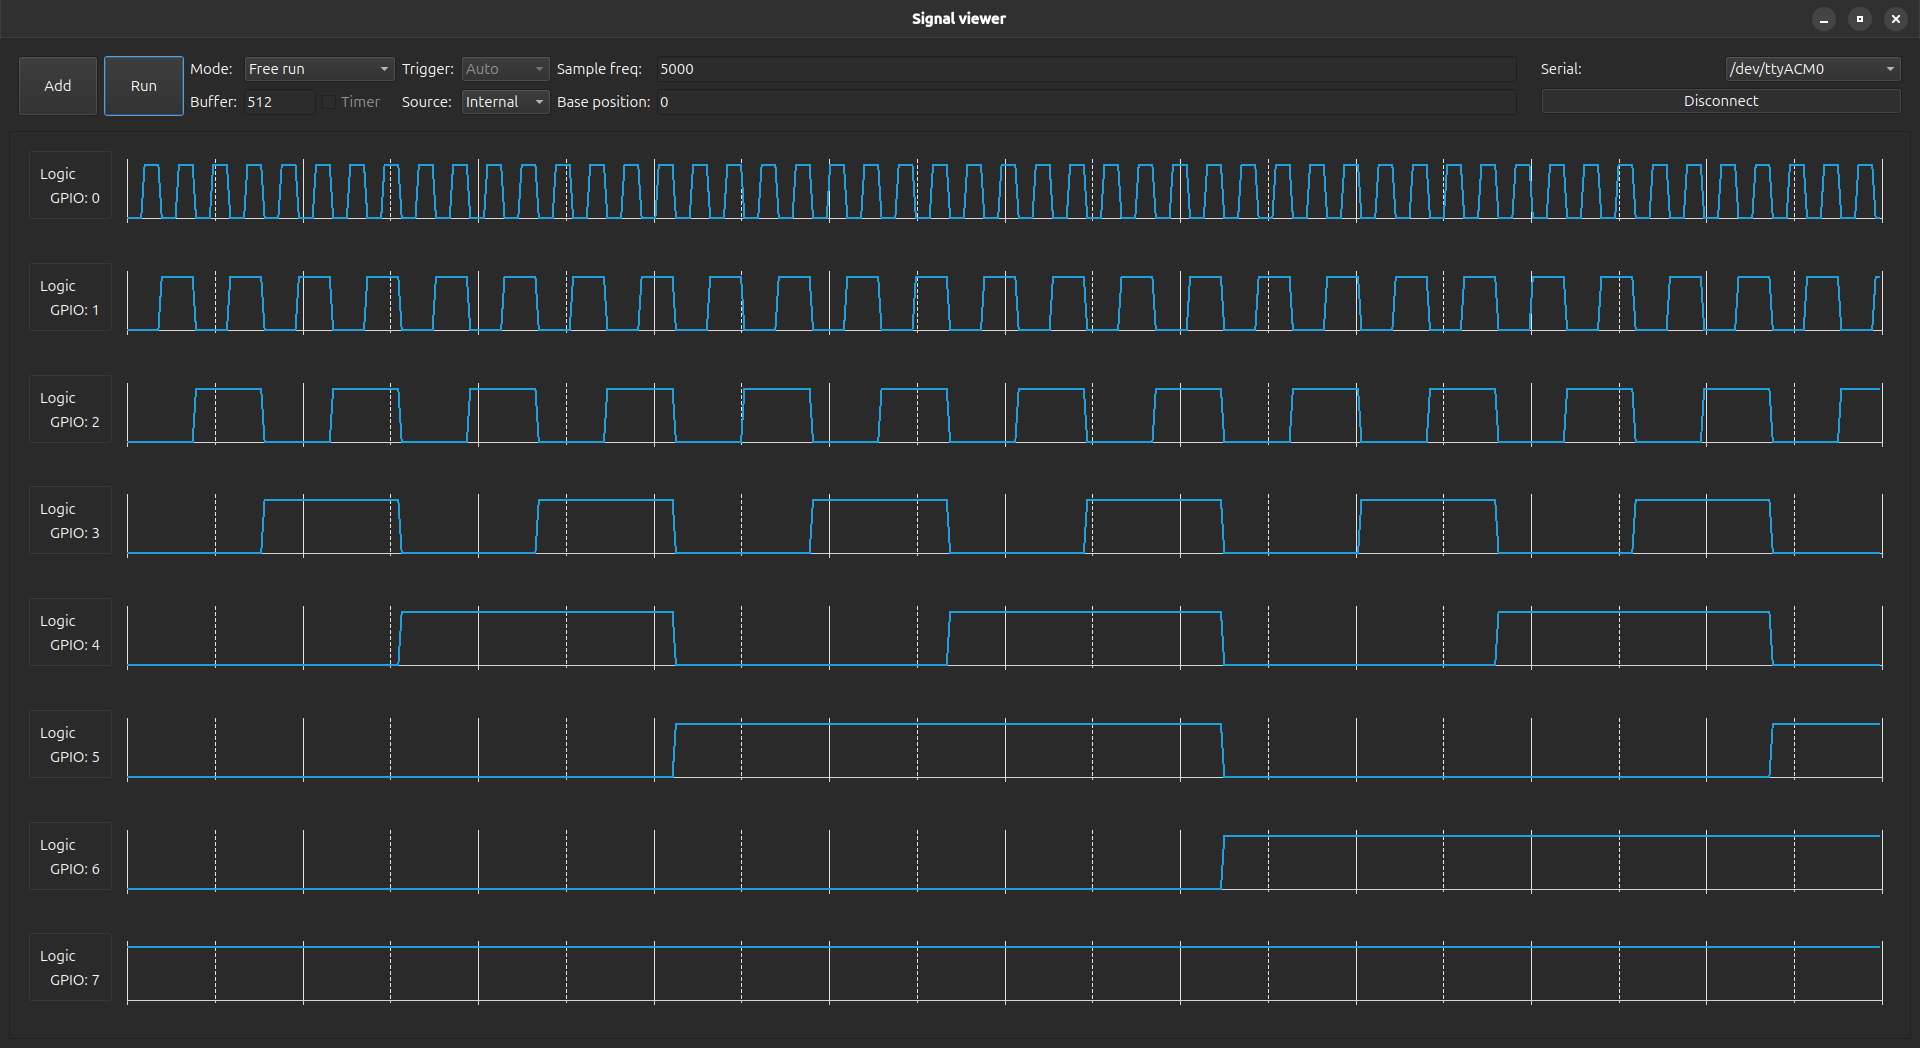
\includegraphics[width=0.8\textwidth]{test_1khz.png}
        \caption{Zdjęcie aplikacji - pomiar testowy, częstotliwość sygnału 1kHz}
    \end{figure}

    Odczytana częstotliwość na podstawie ilości próbek: $f_read = 1kHz$, co odpowiada zadanej częstotliwości wejściowej.